\documentclass{beamer}
%\setbeameroption{show notes}
%\setbeameroption{hide notes}
\setbeamercovered{transparent} 
\usetheme{Warsaw}

\setbeamertemplate{caption}[numbered]
\setbeamertemplate{enumerate items}[default]
\usepackage{copyrightbox}

\usepackage{siunitx}
\DeclareSIUnit\solarmass{\ensuremath{M_\odot}}
\DeclareSIUnit \parsec{pc}

\title{Predicting the limits of the ELT}
\subtitle{Defensio}
\author[Alarich Herzner]{Alarich Herzner\\[1ex]  {\small Supervisor: Univ.-Prof. Jo\~ao Alves, PhD \\ Co-Supervisor: Dr. Kieran Leschinski, MSc}}
\institute{University of Vienna, Faculty of Physics}
\date{\today}

\begin{document}
\begin{frame}
\titlepage
\end{frame}

\section{Introduction}

%\subsection{Outline}
%
%\begin{frame}
%\frametitle{Outline}
%\tableofcontents[hideallsubsections] 
%\end{frame}


\subsection{Goals}

\begin{frame}
\begin{block}{Primary objective}
Estimate reliability limit for future IMF studies in the galactic centre using the ELT!
\end{block}
%\vspace{0.5cm}
\end{frame}

\begin{frame}
\frametitle{ELT}
  \begin{figure}
  \copyrightbox[b]{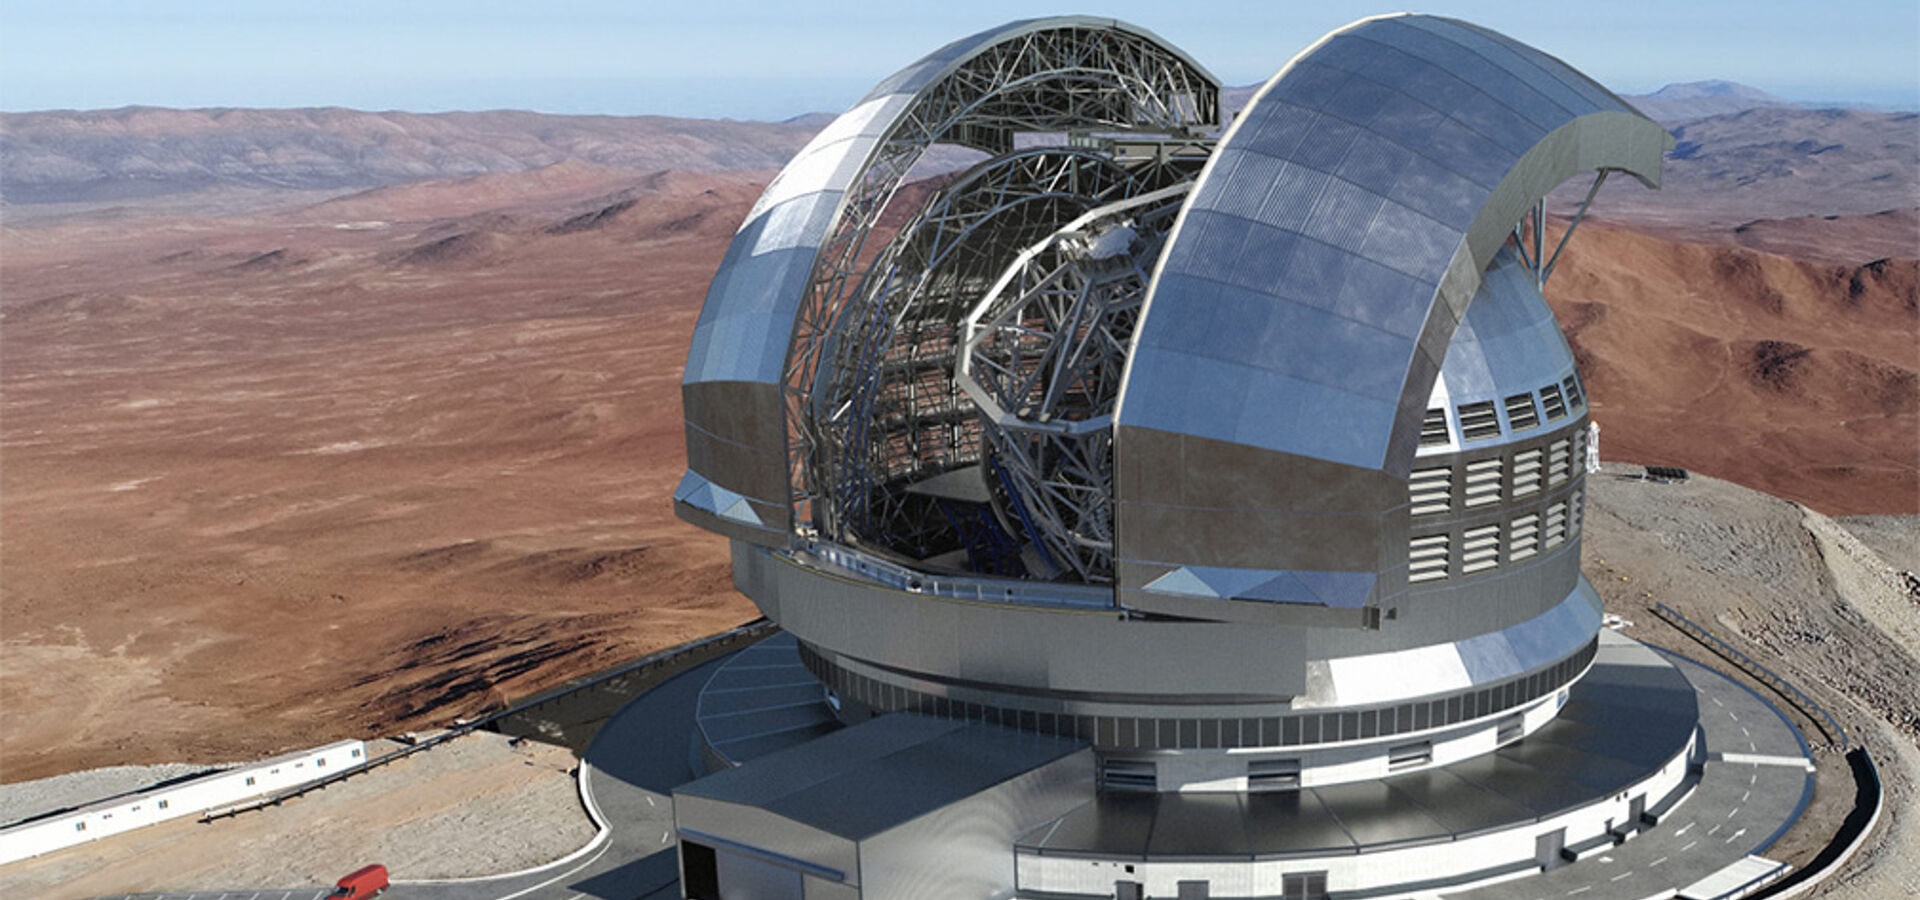
\includegraphics[width=\linewidth]{Images/ELT.jpg}}
                  {https://cdn.eso.org/images/banner1920/telescope-dome-landing.jpg}
  \end{figure}
\end{frame}

\begin{frame}
\frametitle{IMF}
  \begin{figure}
  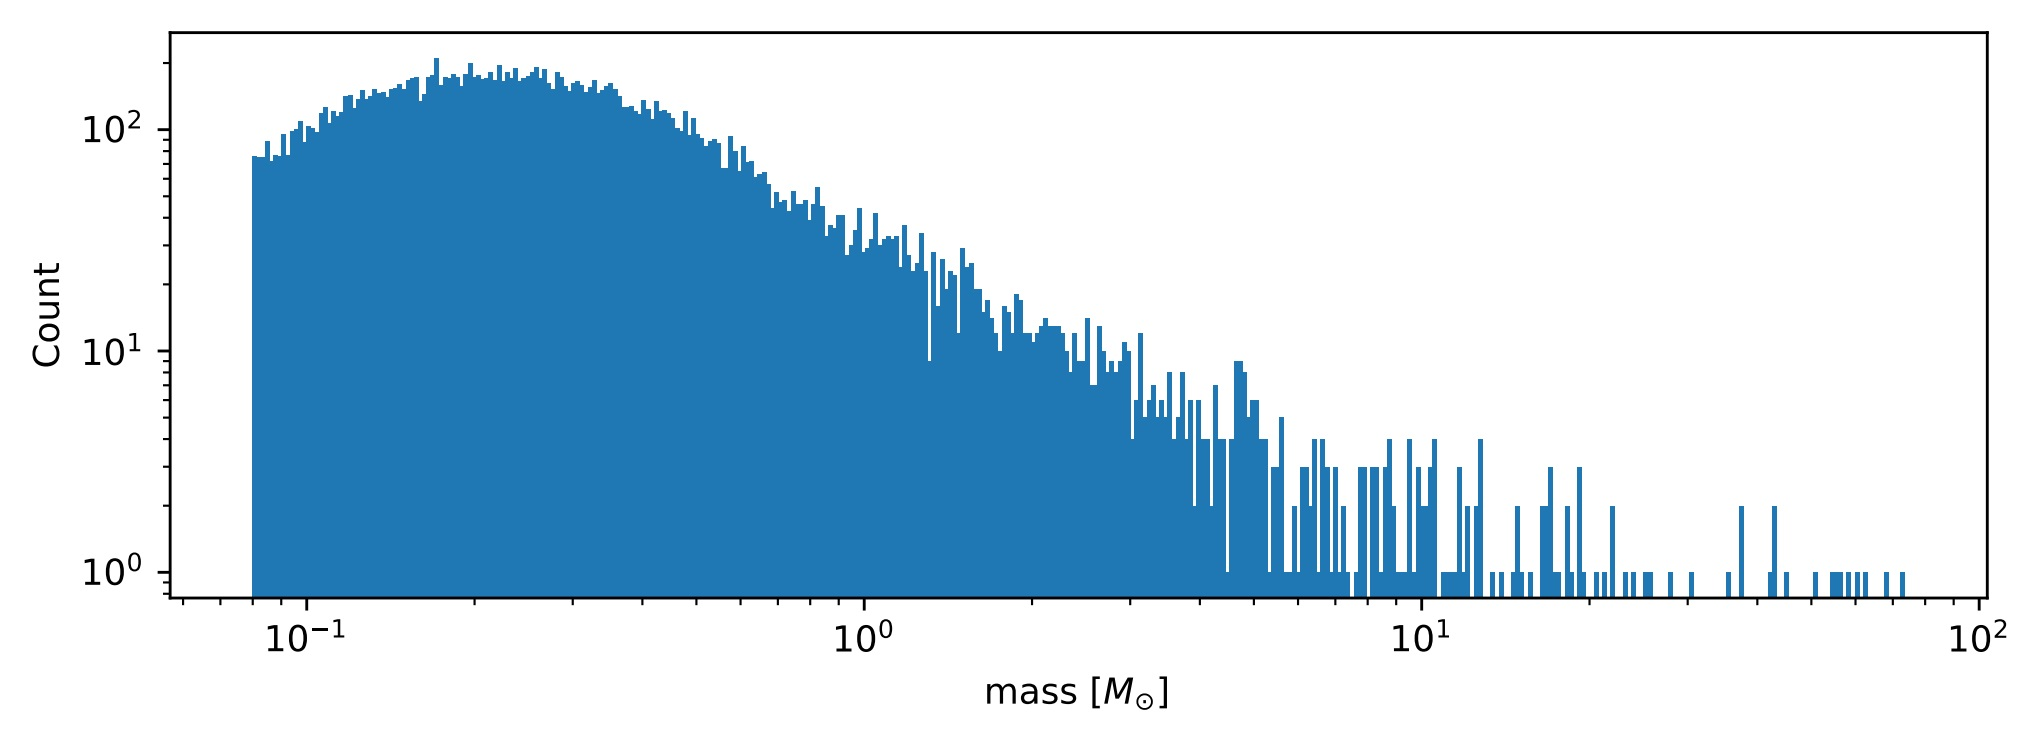
\includegraphics[width=\linewidth]{Images/IMF1.jpg}
  \end{figure}
\end{frame}

\begin{frame}
\frametitle{Reliability Limit}
  \begin{figure}
  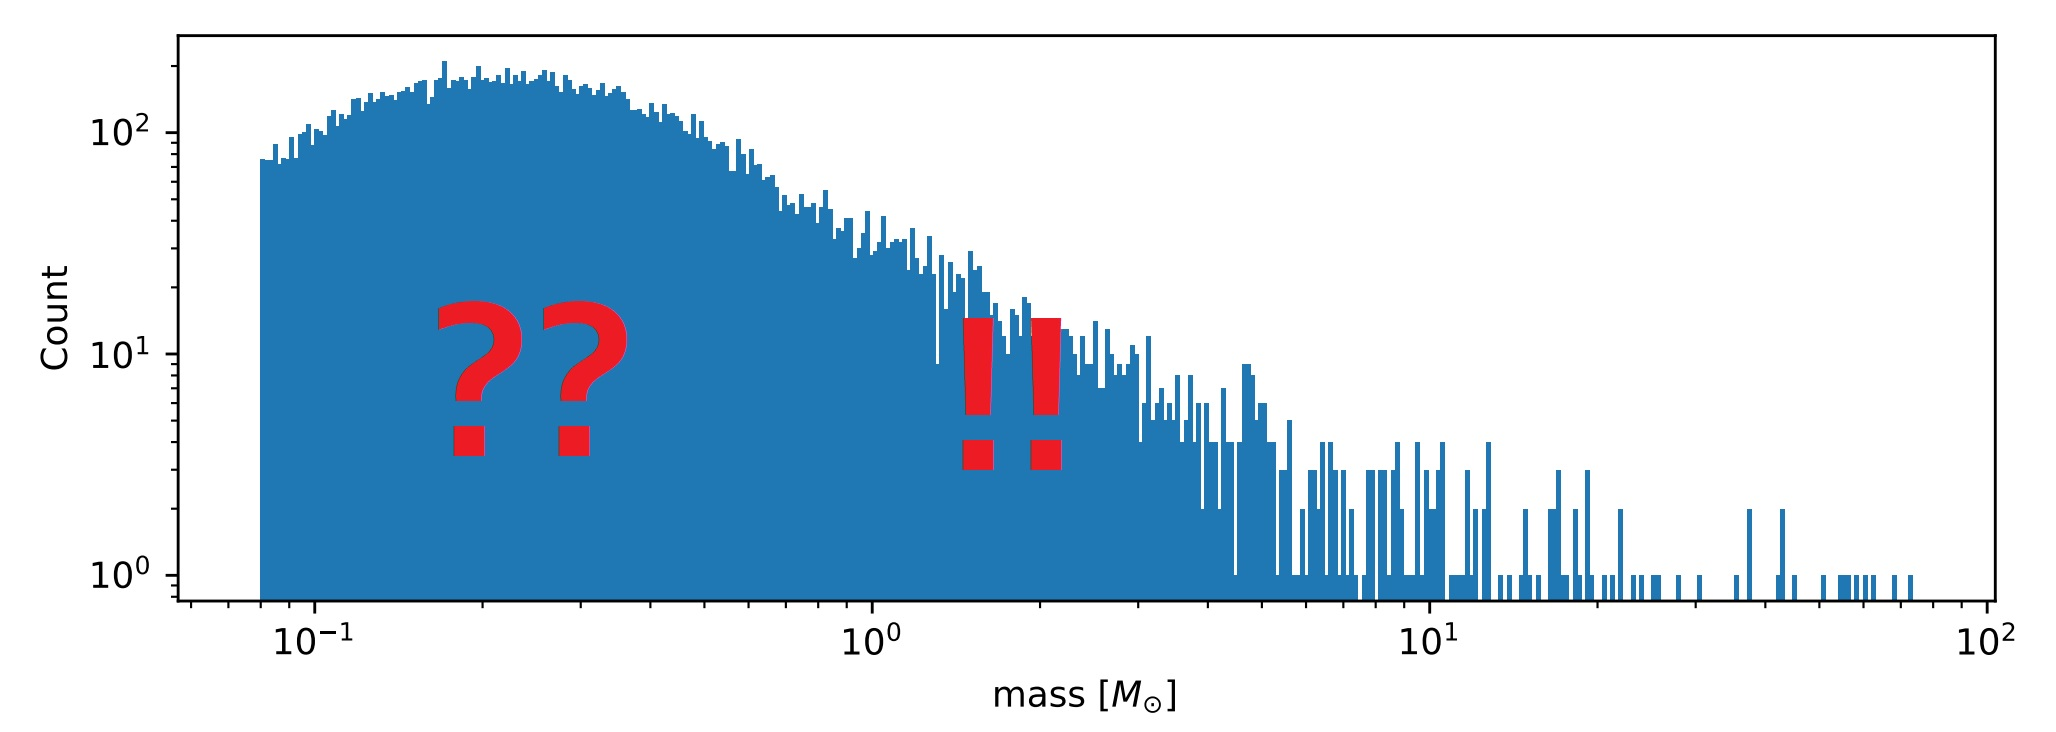
\includegraphics[width=\linewidth]{Images/IMF2.jpg}
  \end{figure}
\end{frame}

\begin{frame}
\frametitle{In other words}
\begin{block}{Primary objective}
Determine reliability of cluster membership detection.
\end{block}
\end{frame}

%\subsection{Motivation}
%
%\begin{frame}
%\begin{block}{Motivation}
%	\begin{columns}[T]
%	\column{0.48\textwidth}
%	\vspace{0.5em}
%	\begin{itemize}
%	\item uncertainty awareness
%	\item baseline reliability
%	\end{itemize}
%	\column{0.48\textwidth}
%	\vspace{0.5em}
%	\begin{itemize}
%	\item N-body simulation \(N \gg 1\)
%	\item Clustering time-dependent data
%	\end{itemize}
%	\end{columns}
%\end{block}
%\end{frame}


%\subsection{Action Plan}
%
%\begin{frame}
%\frametitle{Action Plan}
%\begin{enumerate}
%\item Simulate stars
%\item Observe stars
%\item Analyze
%\item Measure performance
%\end{enumerate}
%\end{frame}

\section{Simulation}

\subsection{Data storage}

\begin{frame}
\begin{figure}
\centering
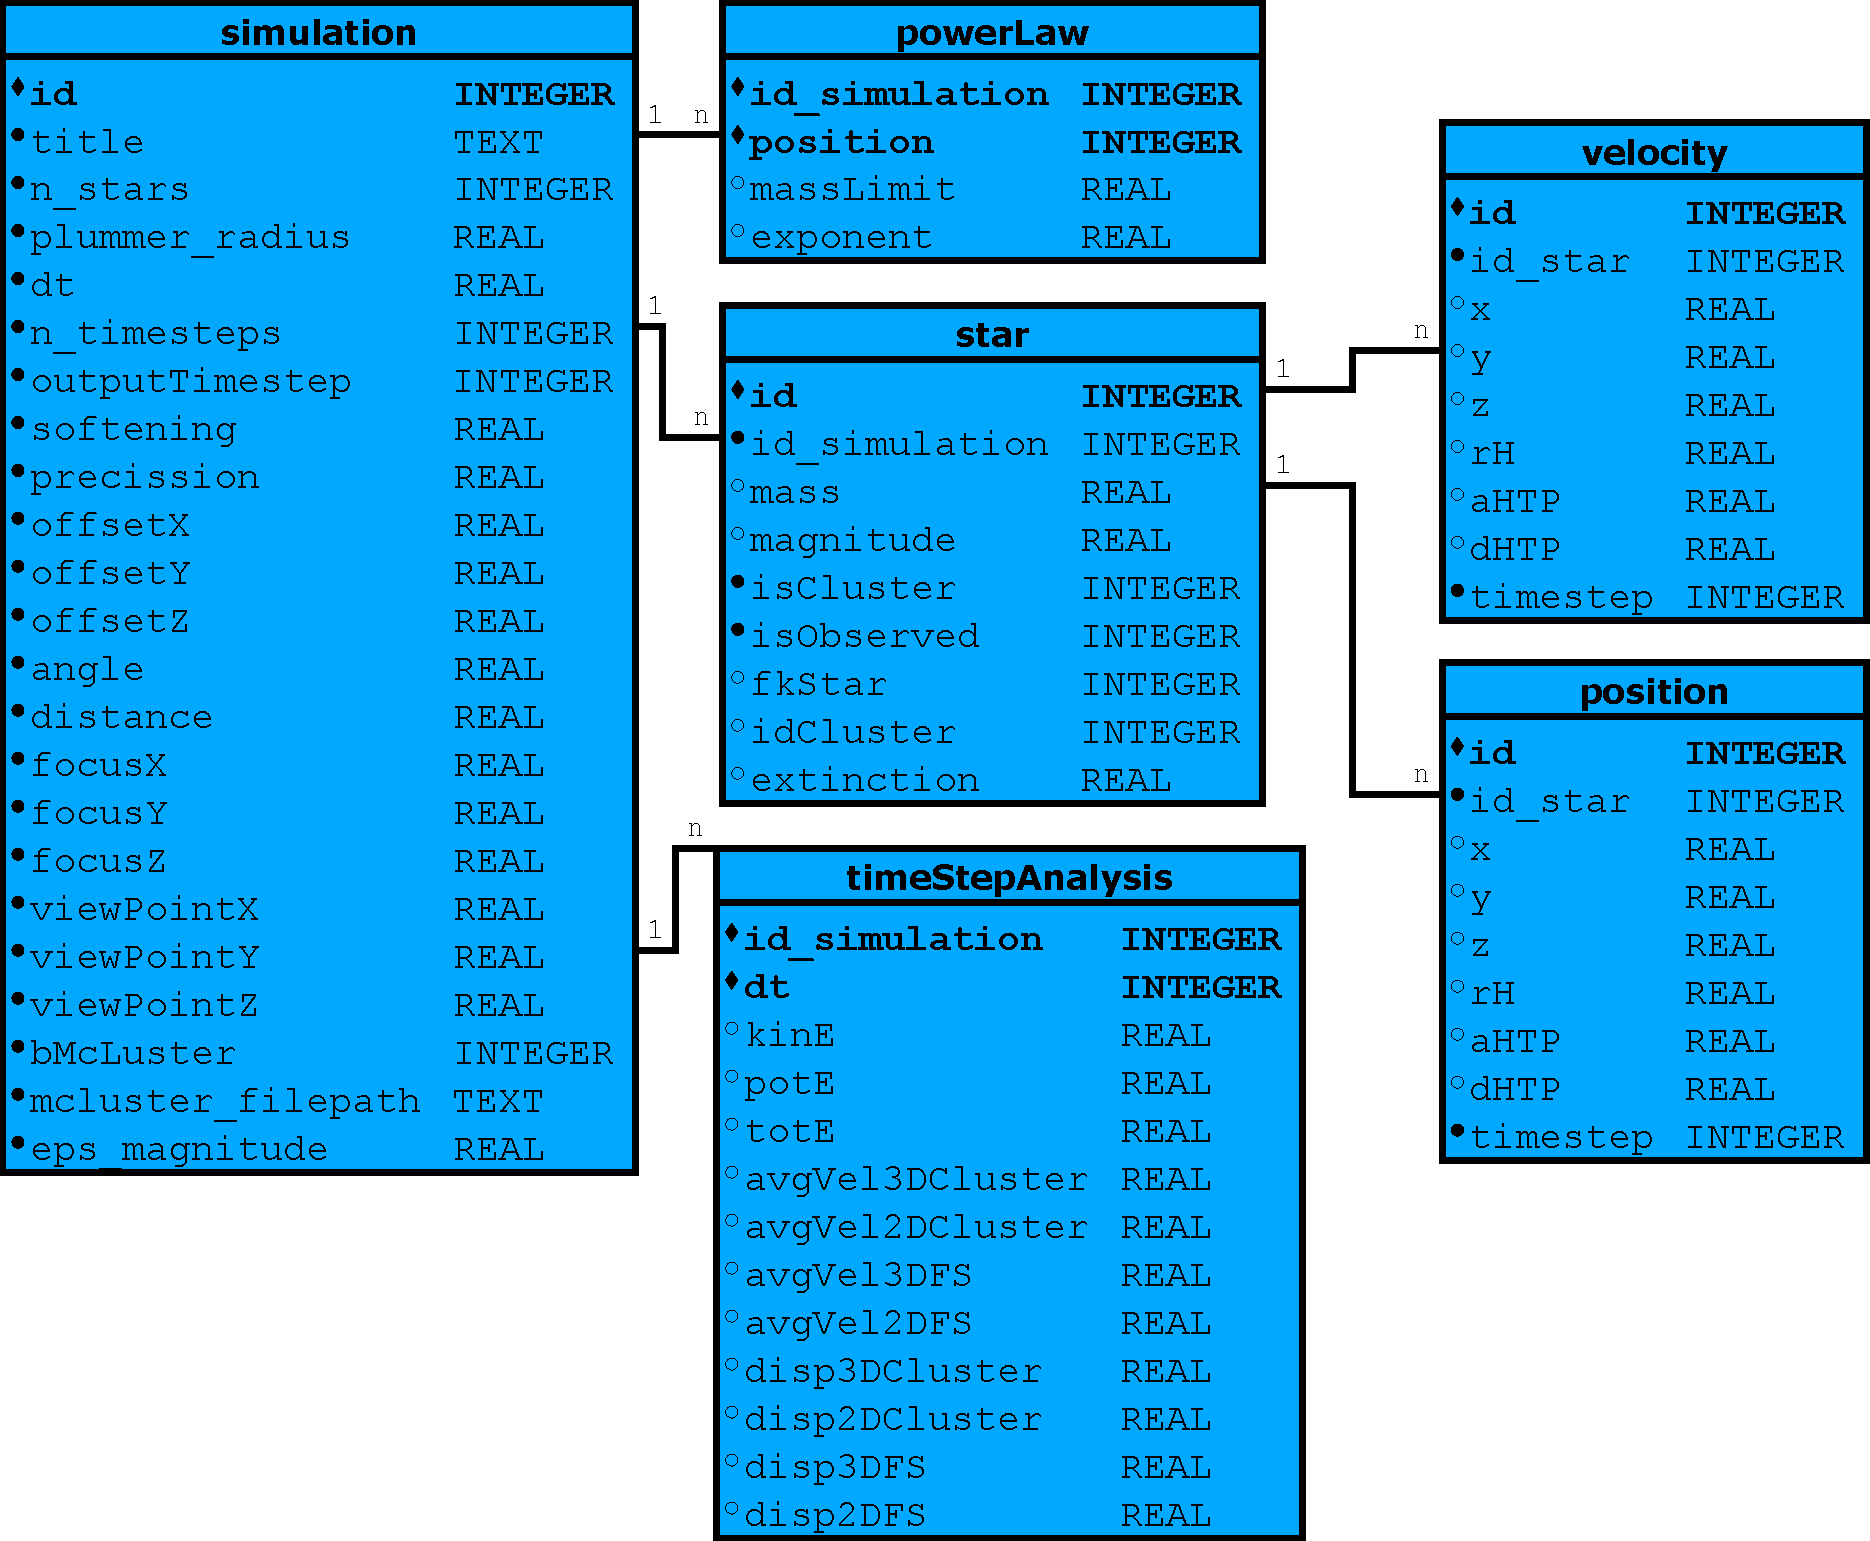
\includegraphics[width=\textwidth,height=0.8\textheight,keepaspectratio]{Images/ERD.pdf}
\end{figure}
\end{frame}


\subsection{Cluster}

\begin{frame}
\frametitle{Initialize star cluster}
McLuster by Andreas Kuepper with Kroupa, P. \& Baumgardt, H.
\\[2ex]
\begin{itemize}
\item<1-> Plummer density profile
\item<2-> virial equilibrium
\item<3-> Kroupa IMF \SIrange{0.08}{100}{\solarmass}
%\item<4-> Metallicity  in range 0.5 - 2 solar
%\item<5-> No binaries
\item<4-> N 1.3k - 40.4k
\end{itemize}

\end{frame}

\begin{frame}
\frametitle{Force Calculation}

\begin{itemize}
\item<1-> Direct summation \(O(N^2)\)
\item<2-> Barnes-Hut Algorithm \(O(N\log(N))\)
	\begin{itemize}
	 \item approximate with macro particles
	 \item \(\frac{width}{distance} < \theta_{max}\)
	\end{itemize}
%\item<3-> Softening
%\item<4-> Time step size
\end{itemize}

\end{frame}


%\begin{frame}
%\begin{figure}
%\centering
%\copyrightbox[b]{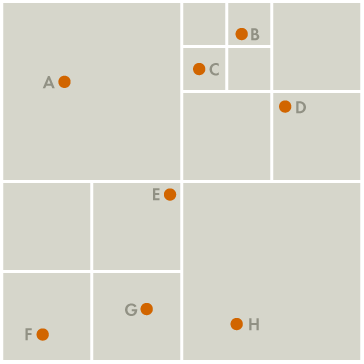
\includegraphics[width=0.65\linewidth]{Images/bh1.png}}
%                  {http://arborjs.org/docs/img/example-space.png}
%\end{figure}
%\end{frame}

\begin{frame}
\begin{figure}
\centering
\includegraphics[width=0.9\linewidth]{Images/Barnes–Hut check_1000.png}
\end{figure}
\end{frame}


\subsection{Milky Way Potential}

\begin{frame}

Multi-component axis-symmetric potential \(\Phi \left ( R,z \right )\) and density.

\begin{itemize}
\item<1-> needed for
	\begin{itemize}
	\item Force from analytic derivatives
	\item Initial conditions for field stars
	\end{itemize}
\item<2-> components
	\begin{itemize}
	\item Black hole: Keplerian potential \(\Phi_{bh} \left ( r \right )\)
	\item Disk: Miyamoto Nagai potential \(\Phi_{disk} \left ( R,z \right )\)
	\item Bulge: Hernquist potential \(\Phi_{bulge} \left ( r\right )\)
	\item Dark matter halo: Navarro–Frenk–White potential \(\Phi_{halo} \left ( r \right )\)
	\end{itemize}
\end{itemize}

\end{frame}

\subsection{Cone of vision}

\begin{frame}
\begin{figure}
\centering
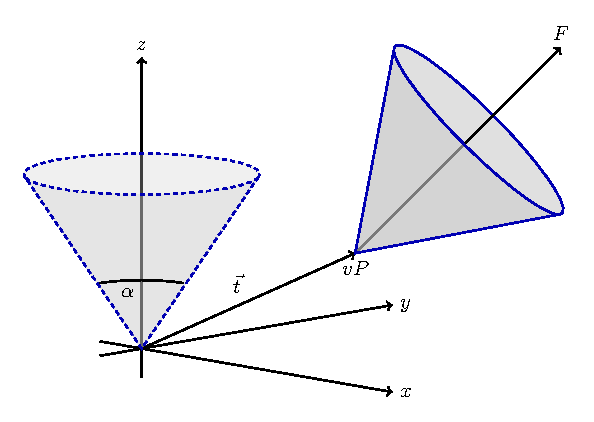
\includegraphics[width=0.9\linewidth]{Images/cone.pdf}
\end{figure}
\end{frame}

\subsection{Field stars}

\begin{frame}
\frametitle{Initialize field stars}
\begin{enumerate}
\item Total mass inside code
\item Sample mass functions N 0.7k - 351.2k
\item Positions: sample density
\item Velocities: Jeans equations
\end{enumerate}
%\begin{equation*}
%M = \int_{-R}^{R}\int_{-\sqrt{R^2-x^2}}^{\sqrt{R^2-x^2}}\int_{\frac{h}{R}r}^{h} \rho \left ( \mathbf{T} \cdot \begin{pmatrix}x\\ y\\ z\end{pmatrix} \right ) dzdydx
%\end{equation*}

%\begin{description}
%\item[\(R\)] cone base radius
%\item[\(T\)] transformation matrix
%\item[\(h\)] cone height
%\end{description}

%Integration

%\begin{itemize}
%\item GSL: GNU Scientific Library
%\item Gauss-Kronrod quadrature
%\end{itemize}

\end{frame}


%\begin{frame}
%\frametitle{Initialize mass (2)}

%Sample mass functions

%\begin{itemize}
%\item rejection sampling
%\item inverse transformation sampling
%\item N 0.7k - 351.2k
%\end{itemize}

%\begin{figure}
%\centering
%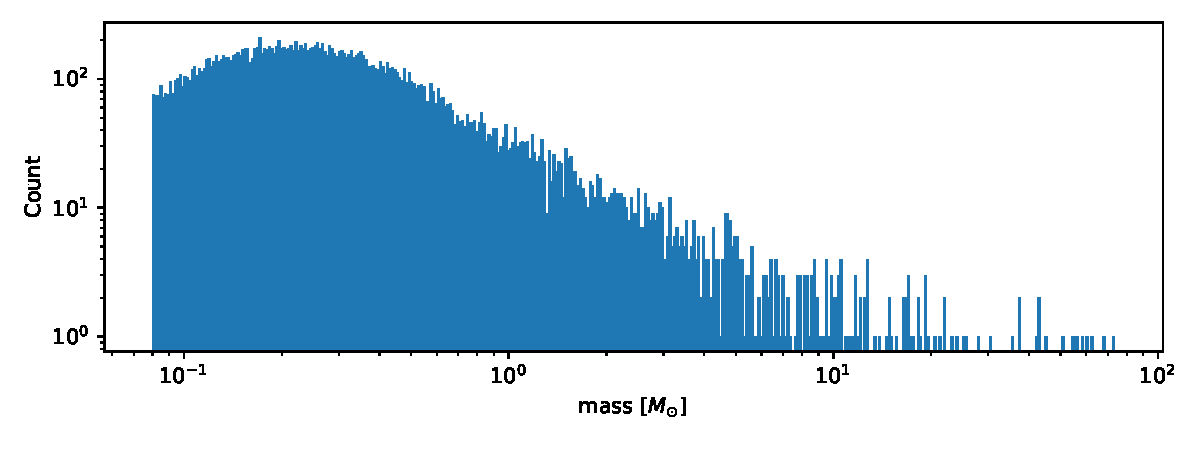
\includegraphics[width=\linewidth]{Images/initial_conditions_mass_bulge.pdf}
%\end{figure}

%\end{frame}


\begin{frame}
%\frametitle{Positions}

%\begin{enumerate}
%\item uniform distribution
%\item transformation
%\item rejection sampling
%\end{enumerate}

\begin{figure}
\centering
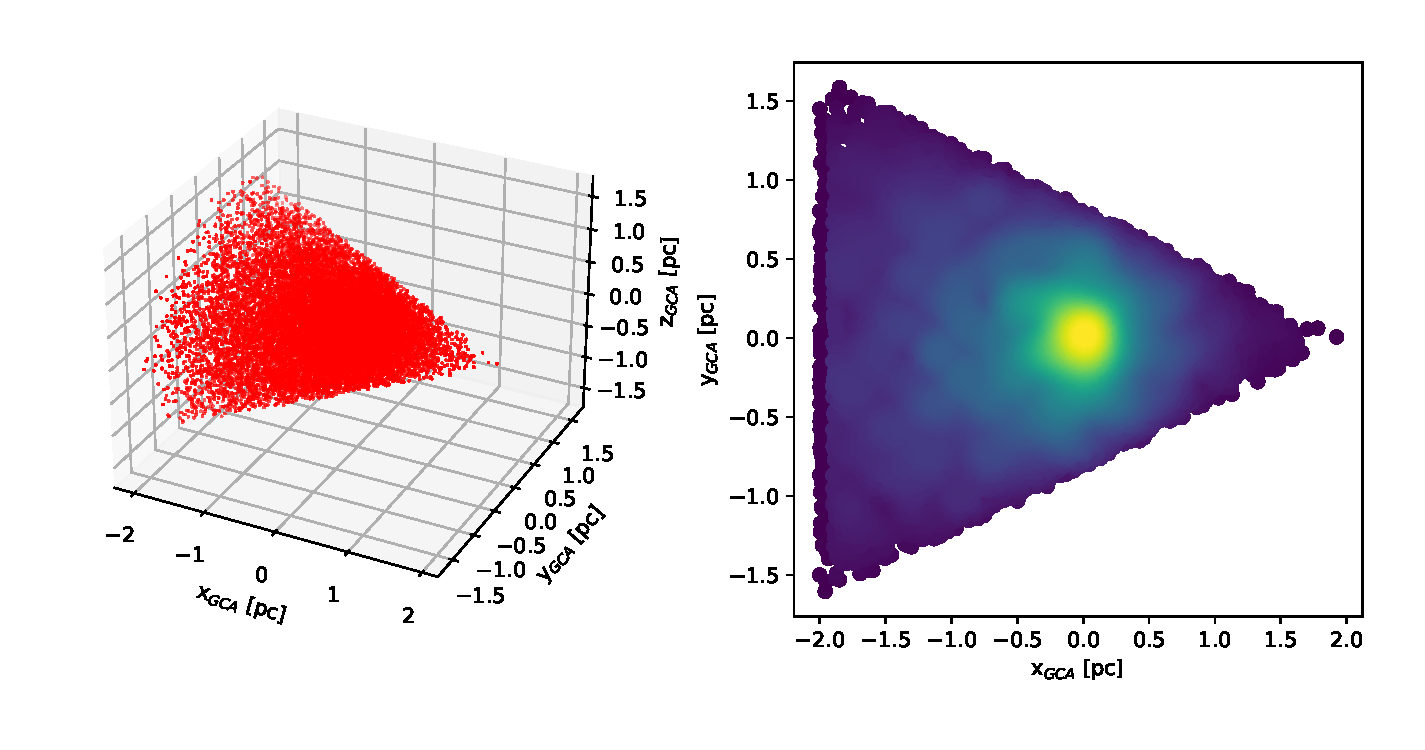
\includegraphics[width=\linewidth]{Images/cone_3D.pdf}
\end{figure}

\end{frame}


%\begin{frame}
%\frametitle{Velocities}

%Solve Jeans equations + constraints from observations

%\begin{itemize}
%\item Disk
%	\begin{itemize}
%	\item Epicyclic Approximation
%	\item average \& dispersion
%	\item Sampled from Gaussian distributions
%	\end{itemize}
%\item Bulge
%	\begin{itemize}
%	\item \(\sigma_r^2 = \frac{1}{\rho}\int_{r}^{\infty}\rho \frac{\partial \Phi}{\partial r}\textup{dr}\)
%	\item Lookup table
%	\item isotropic
%	\item limited by escape speed
%	\end{itemize}
%\end{itemize}

%\end{frame}

\begin{frame}
\begin{figure}
\centering
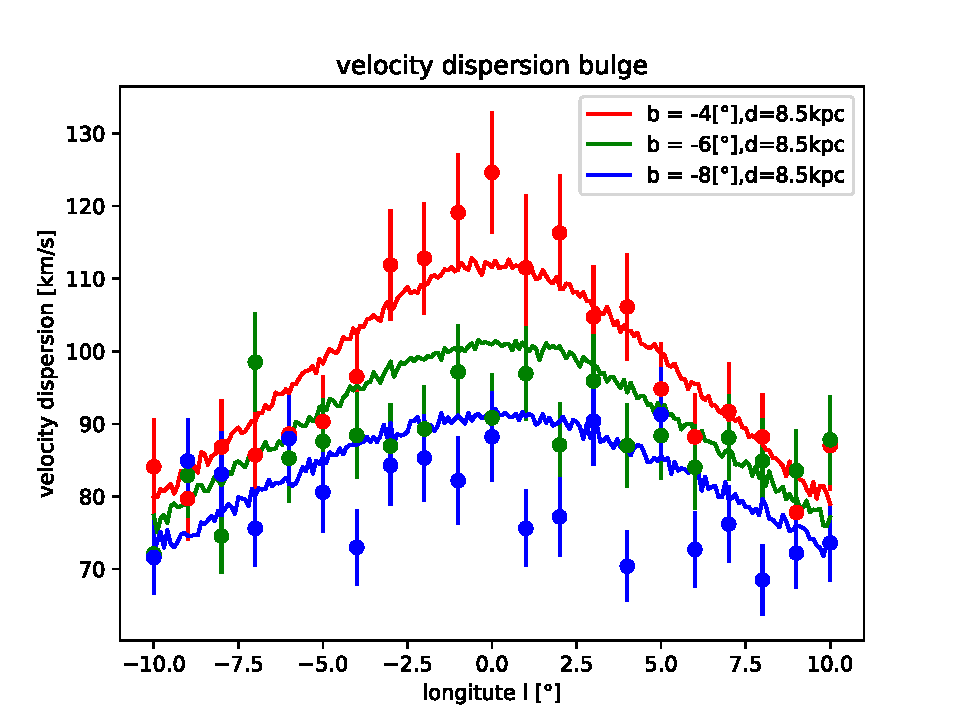
\includegraphics[width=\textwidth,height=\textheight,keepaspectratio]{Images/velocity_dispersion_bulge.pdf}
\end{figure}
\end{frame}


\begin{frame}
\begin{enumerate}
\item<1-> Integrate equations of motion
%	\begin{itemize}
%	\item Euler
%	\item Velocity Verlet
%	\end{itemize}
\item<2-> Write to Database
\item<3-> Test total Energy
%\item<4-> Boundary conditions?
\end{enumerate}
\end{frame}


\begin{frame}
\begin{figure}
\centering
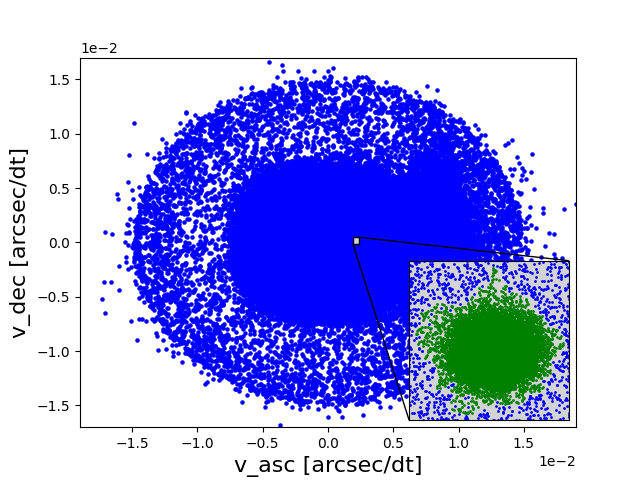
\includegraphics[width=\textwidth,height=0.8\textheight,keepaspectratio]{Images/title_page.png}
\end{figure}
\end{frame}

\section{Observation}

\subsection{Coordinate Systems}

\begin{frame}
\frametitle{Coordinate Systems}

GalPot by Paul McMillan
\\[2ex]
\begin{description}
\item[GCA] Galactocentric Cartesian
\item[LSR] Local Standard of Rest
\item[HCA] Heliocentric Cartesian
\item[HTP] Heliocentric Telescope Polar
\end{description}

\end{frame}

\subsection{Snapshots}

\begin{frame}

ScopeSim by Kieran Leschinski
\\[2ex]
Spectra
\begin{itemize}
%\item Spectral type
\item Pickles catalogue
\item From mass and distance
%\item Apparent magnitude
\item Extinction
%\item Weight of spectrum
\end{itemize}
\vspace{\baselineskip}
Output FITS files
\end{frame}

\begin{frame}
\begin{figure}
\centering
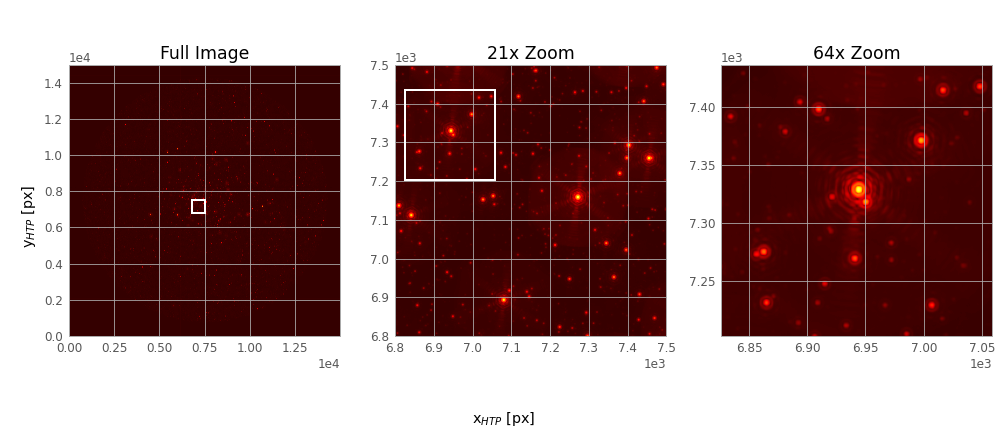
\includegraphics[width=\textwidth]{Images/fits_snapshot.png}
\end{figure}
\end{frame}

\subsection{Source Detection}

\begin{frame}
Photutils by Larry Bradley et al.
\\[2ex]
\begin{itemize}
\item DAOStarFinder
	\begin{itemize}
	\item Threshold
	%\item 2D Gaussian kernel
	\item Roundness
	\item Mask
	\end{itemize}

%\item<2-> Image Segmentation
%	\begin{itemize}
%	\item Connected pixels 
%	\item Threshold
%	\item Source Deblending
%	\end{itemize}
\end{itemize}
\end{frame}


\begin{frame}
\begin{figure}
\centering
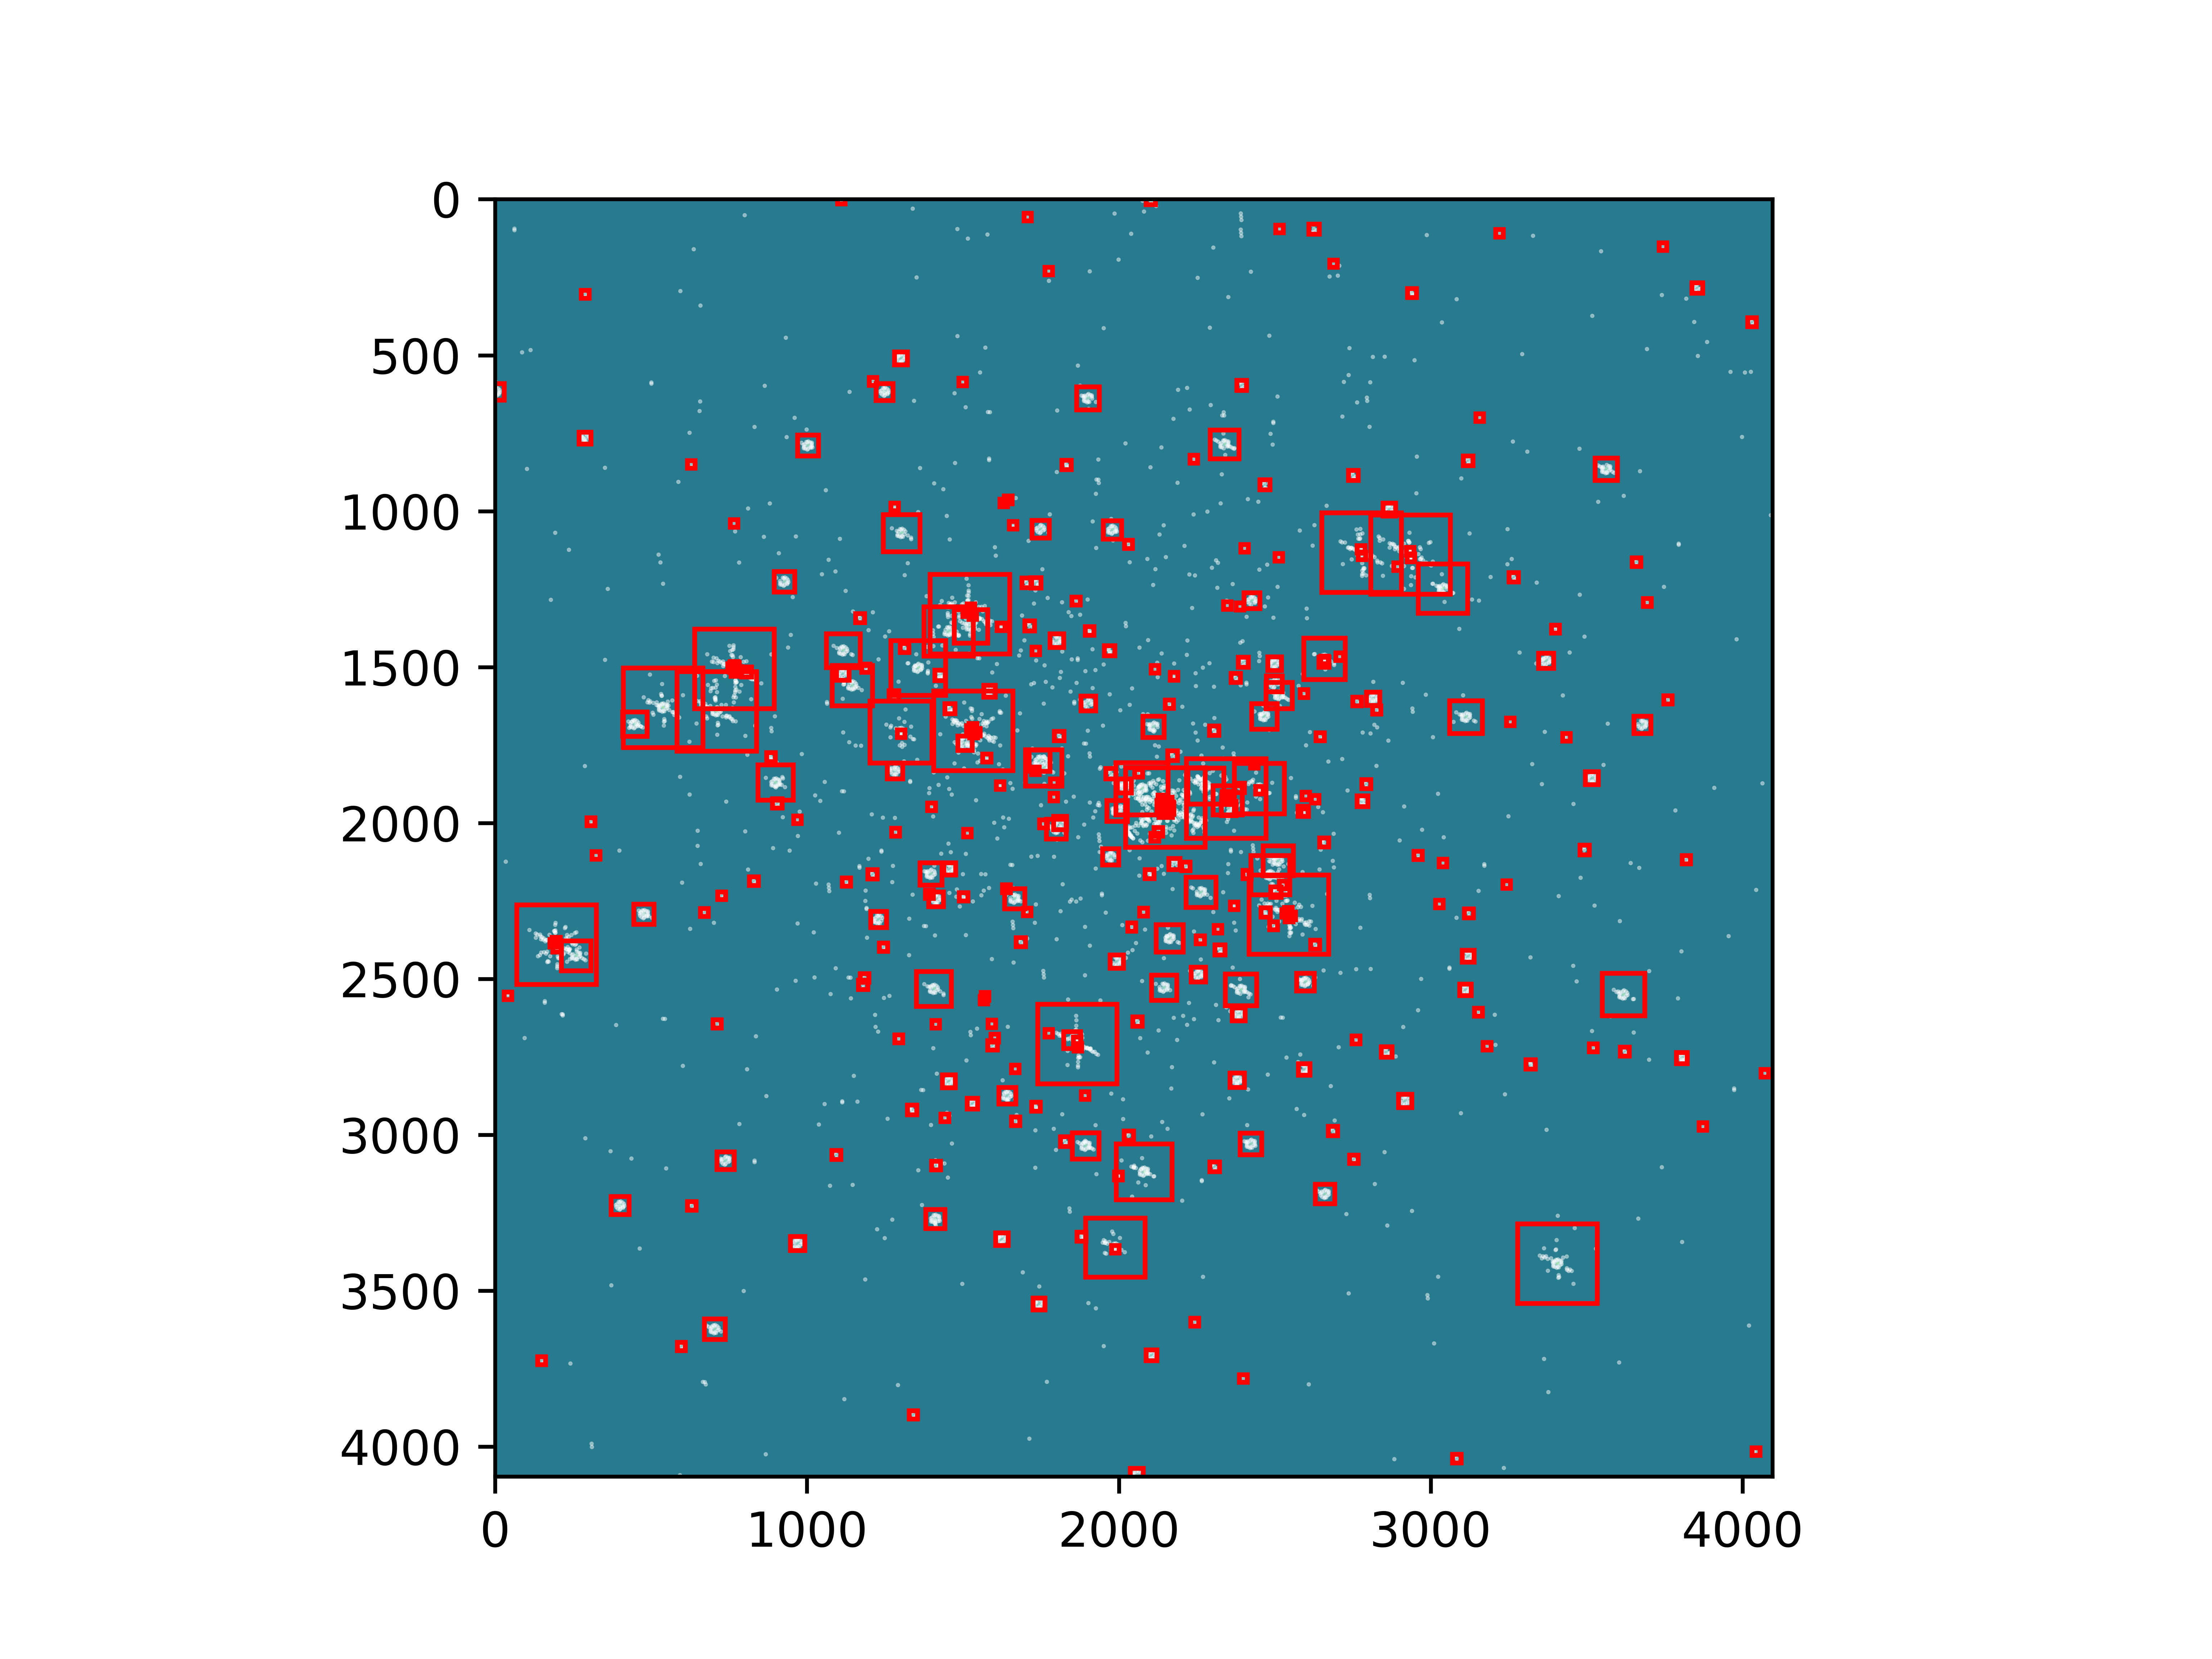
\includegraphics[width=\textwidth,height=\textheight,keepaspectratio]{Images/masking.png}
\end{figure}
\end{frame}


%\begin{frame}
%\begin{figure}
%\centering
%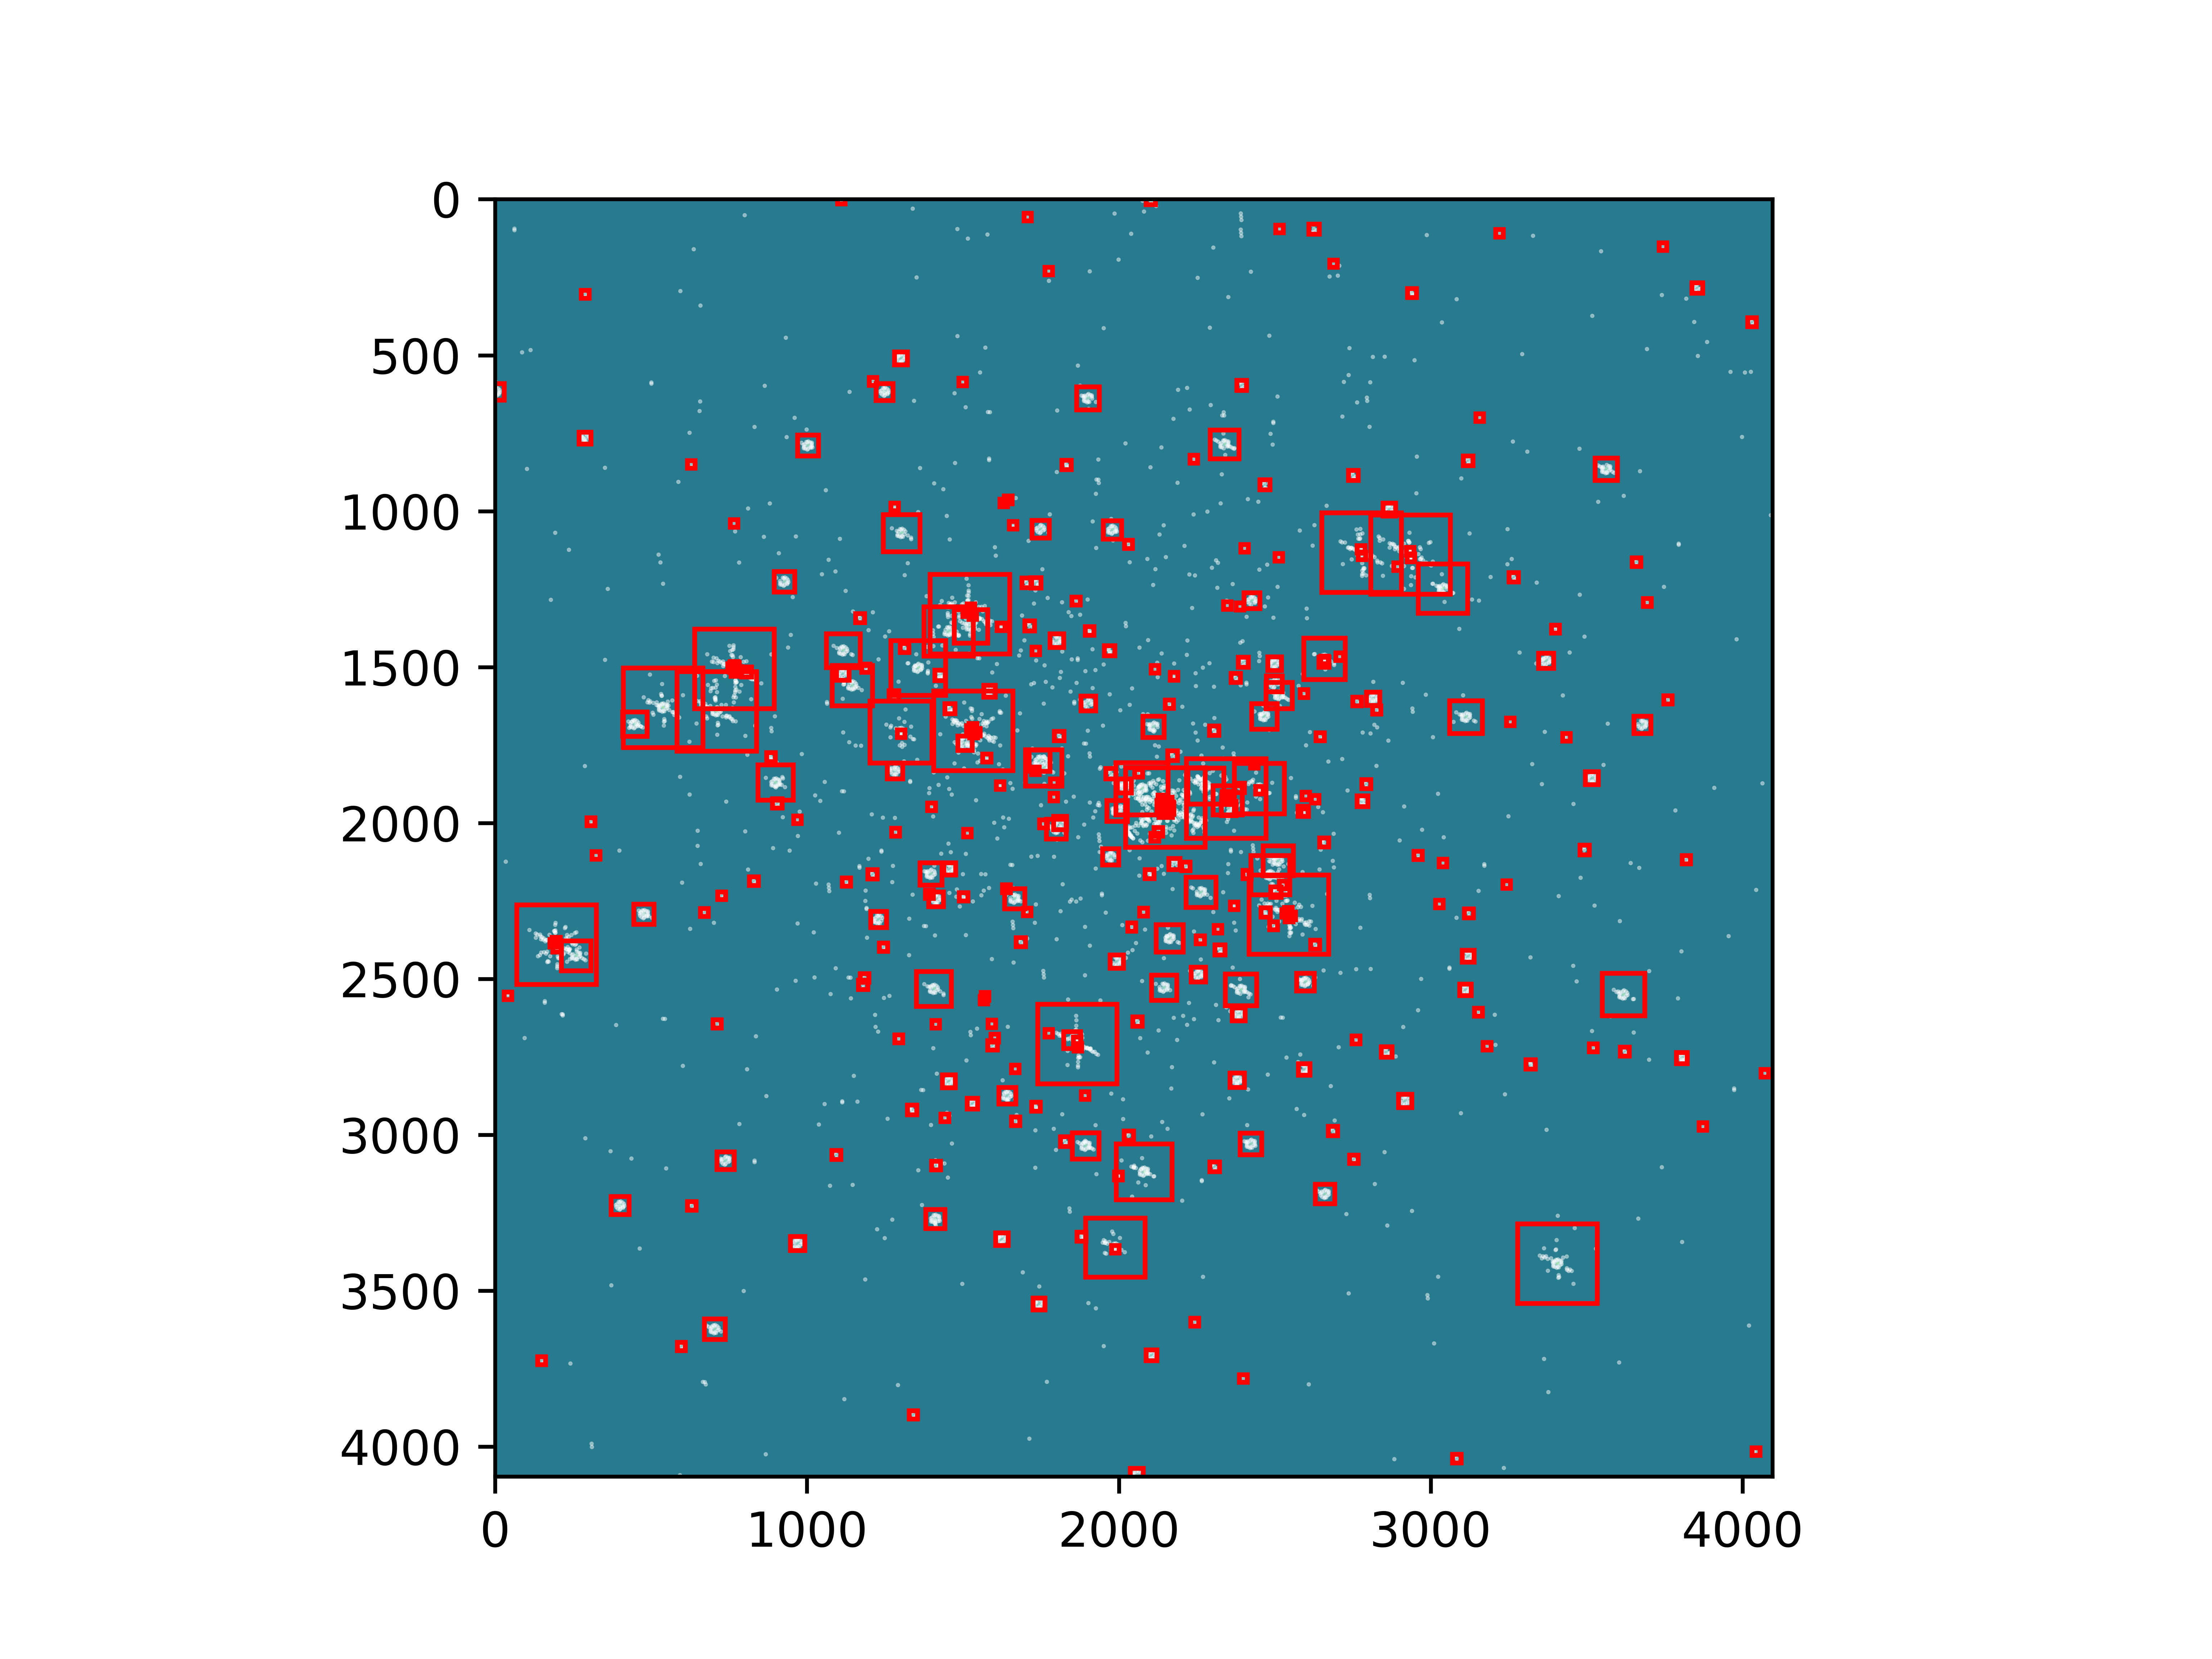
\includegraphics[width=\textwidth,height=\textheight,keepaspectratio]{Images/masking.png}
%\end{figure}
%\end{frame}


\begin{frame}
\begin{figure}
\centering
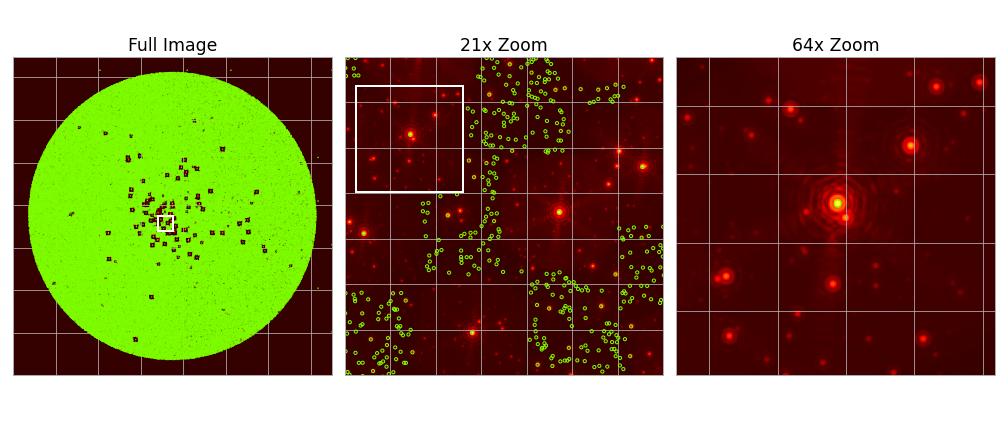
\includegraphics[width=\textwidth,height=\textheight,keepaspectratio]{Images/fits_extracted.png}
\end{figure}
\end{frame}

\section{Analysis}

\subsection{Preparation}
\begin{frame}

mlpack by Ryan Curtin et al.
\\[2ex]
\begin{itemize}
\item Map observed stars 
	\begin{itemize}
	\item Range search
	\end{itemize}
\item Velocity approximation
	\begin{itemize}
	\item Nearest-neighbors search
	\item max magnitude difference
	\item compare with mapping
	\end{itemize}
\end{itemize}

\end{frame}

\subsection{Clustering Algorithm}

\begin{frame}

\begin{block}{DBSCAN Algorithm}
Density-based spatial clustering of applications with noise
\end{block}

Pros:
\begin{itemize}
\item noise
\item amount of clusters
\end{itemize}

\end{frame}


\begin{frame}
\frametitle{F1 Score}
\begin{equation*}
F_1 = 2 \frac{P \cdot R}{P+R} = \frac{TP}{TP+0.5(FP+UP+FN)}
\end{equation*}
\vspace{\baselineskip}
\begin{description}
\item[TP] correctly classified as cluster star
\item[FP] wrongly classified as cluster star
\item[UP] not mapped star classified as cluster star
\item[FN] wrongly classified as field star
\end{description}

\end{frame}


\begin{frame}
\frametitle{Results: F1}
\begin{figure}
\centering
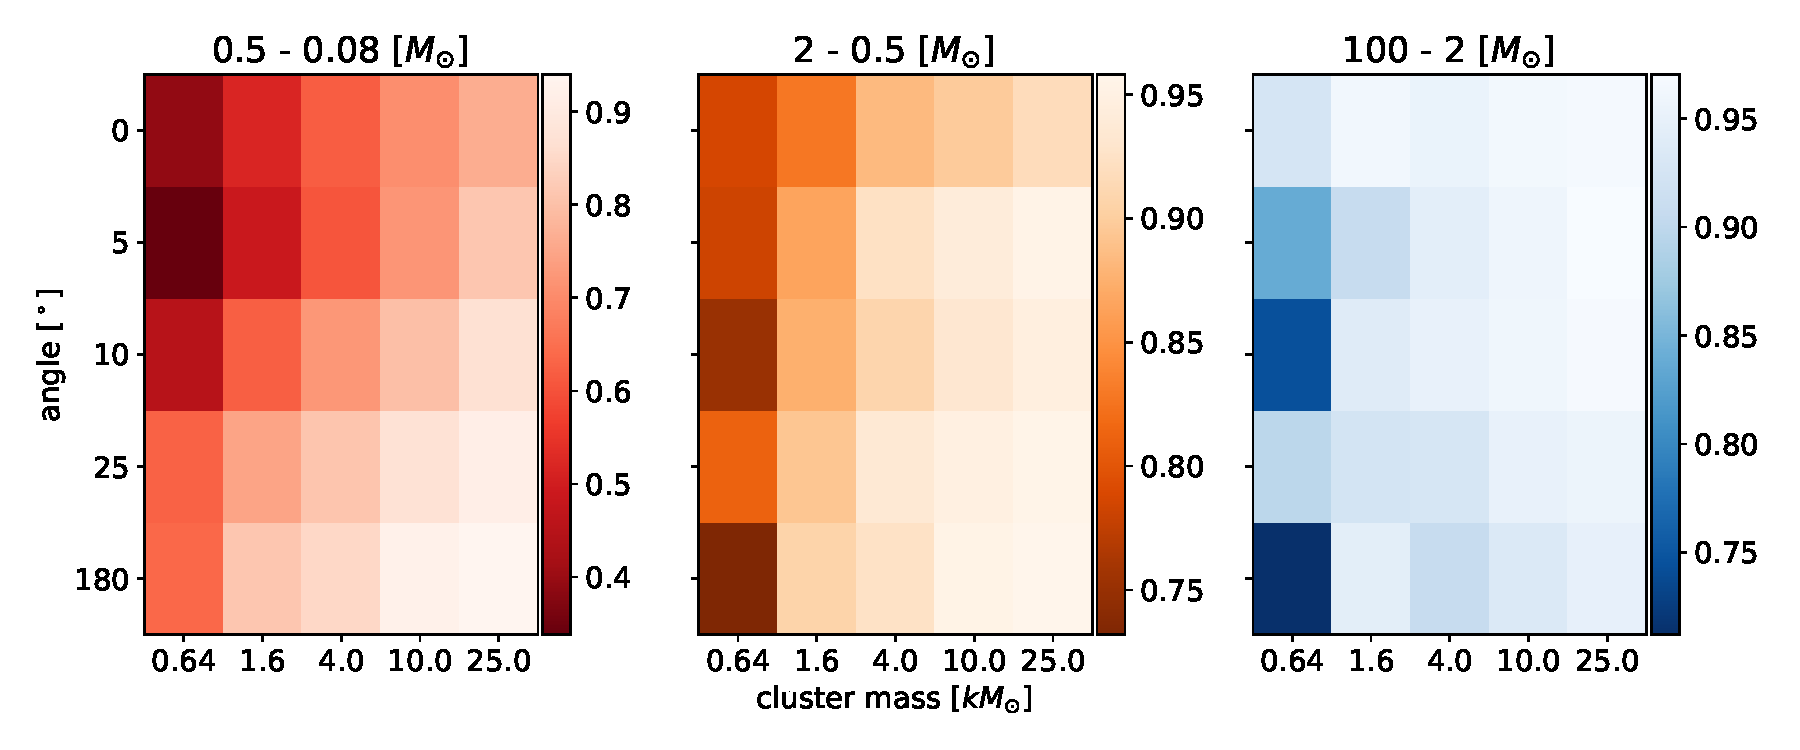
\includegraphics[width=\textwidth,height=\textheight,keepaspectratio]{Images/25_F1.pdf}
\end{figure}

\end{frame}


\begin{frame}
\begin{table}
\centering
\begin{tabular}{|r|r|r|r|}
\hline
Star \si{\solarmass} & Cluster \si{\kilo\solarmass}  & \% Found & F1 Score \\
\hline
<0.5     & 0.64  & 41       & 0.39 \\
<0.5     & 1.60  & 40       & 0.52 \\
<0.5     & 4.00  & 40       & 0.62 \\
<0.5     & 10.00 & 35       & 0.71 \\
<0.5     & 25.00 & 28       & 0.76 \\
0.5 - 2     & 0.64  & 81       & 0.79 \\
0.5 - 2     & 1.60  & 80       & 0.83 \\
0.5 - 2     & 4.00  & 76       & 0.88 \\
0.5 - 2     & 10.00 & 63       & 0.90 \\
0.5 - 2     & 25.00 & 54       & 0.92 \\
\hline
\end{tabular}

\end{table}
\end{frame}

\begin{frame}{}
  \centering \Huge
  \emph{Thank you for your kind attention!}
\end{frame}


% Extra stuff

\begin{frame}
\begin{figure}
\centering
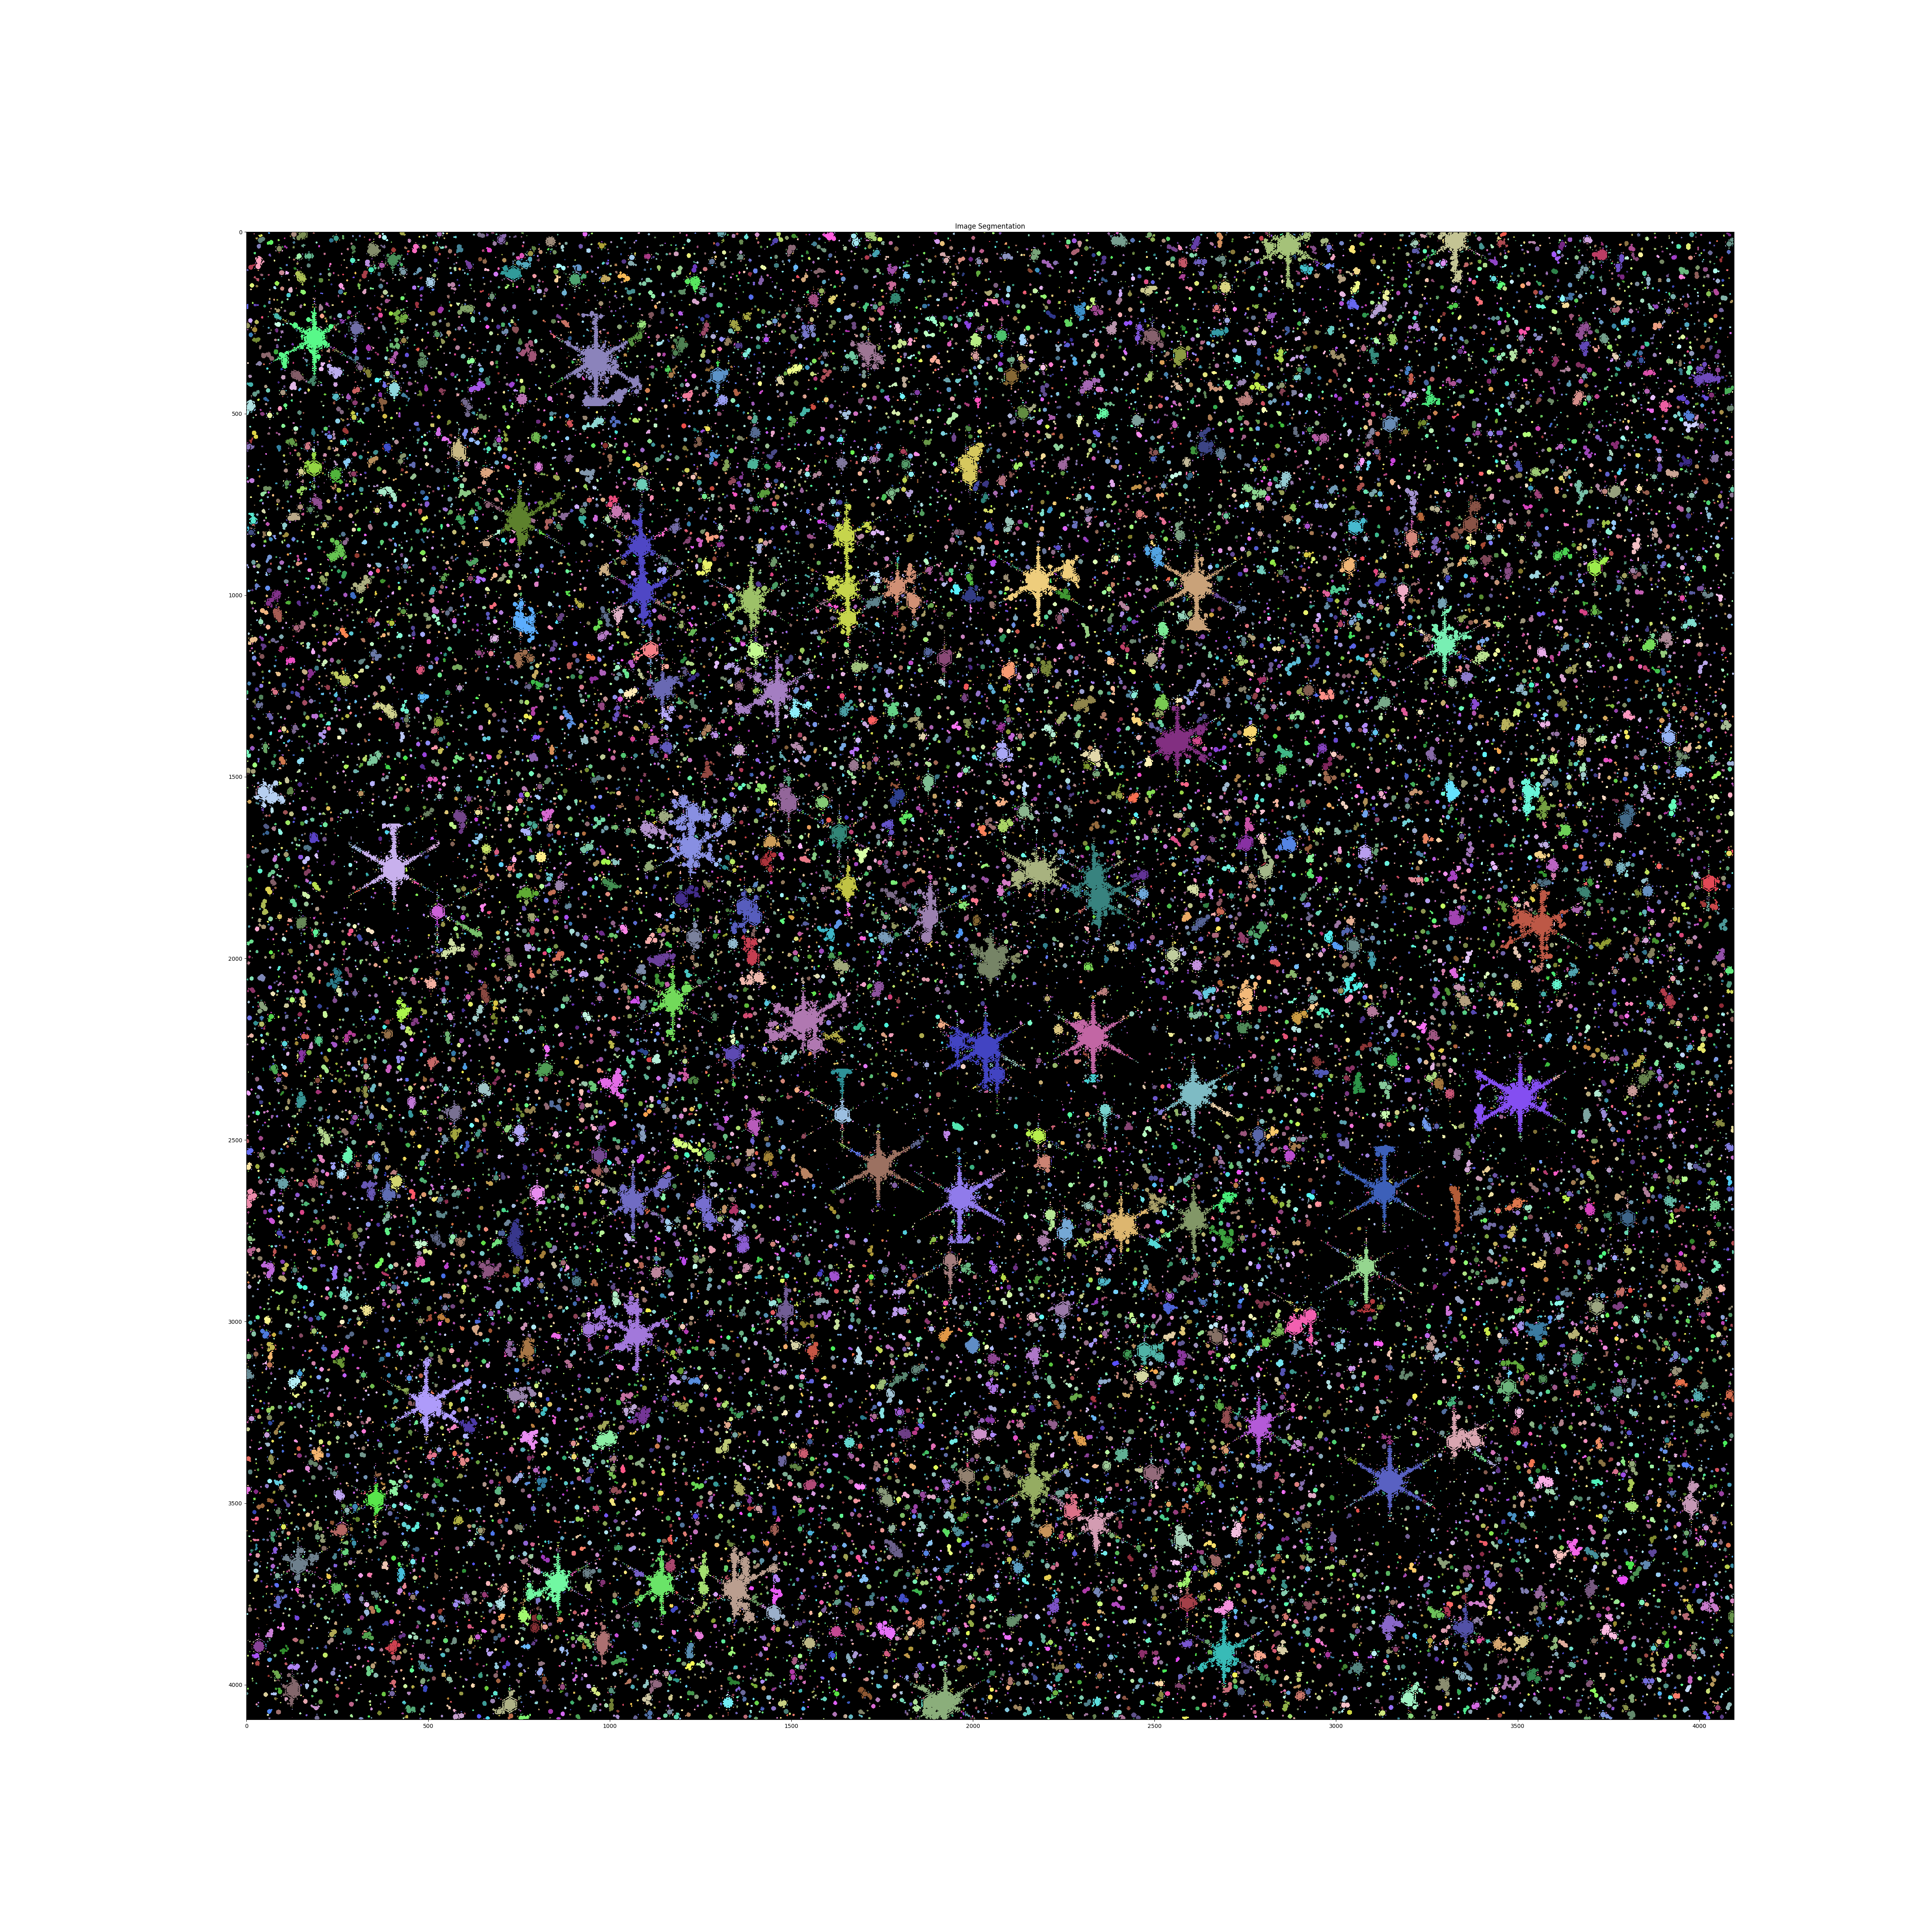
\includegraphics[width=\textwidth,height=\textheight,keepaspectratio]{Images/ISPhotutils_32BK_4THRE_3Kernel.png}
\end{figure}
\end{frame}

\begin{frame}
\begin{figure}
\centering
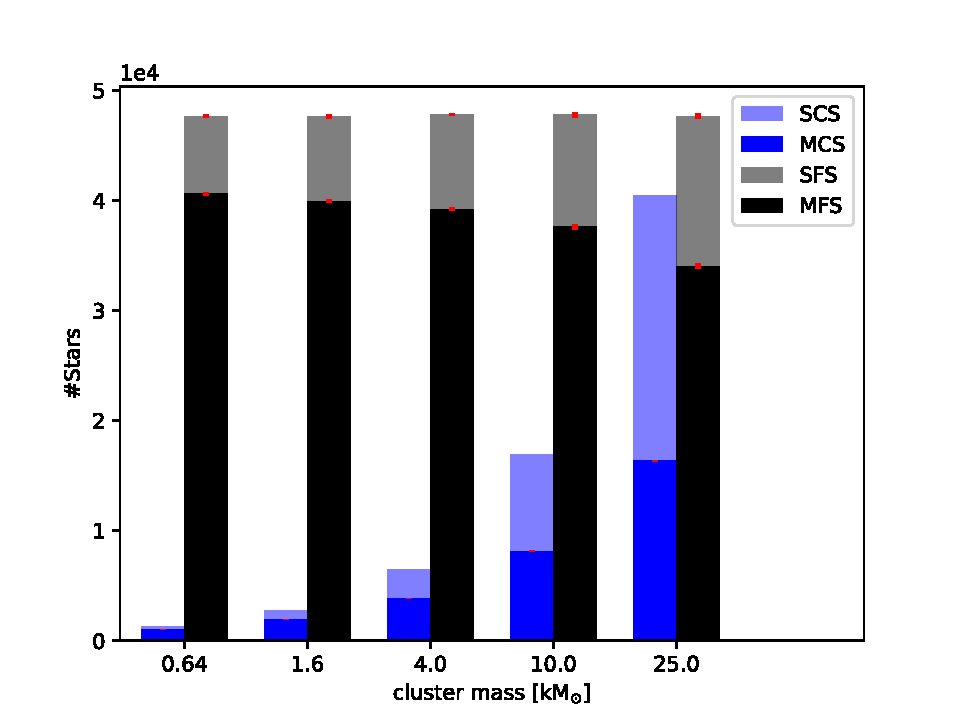
\includegraphics[width=\textwidth,height=\textheight,keepaspectratio]{Images/25_n_stars.pdf}
\end{figure}
\end{frame}

\begin{frame}
\begin{figure}
\centering
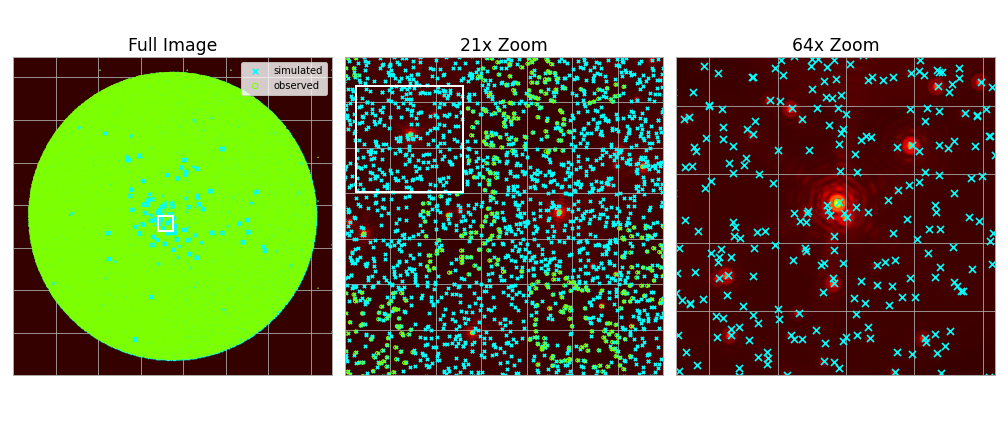
\includegraphics[width=\textwidth,height=\textheight,keepaspectratio]{Images/fits_sim_obs.png}
\end{figure}
\end{frame}

\begin{frame}
\begin{figure}
\centering
\frametitle{Precision}
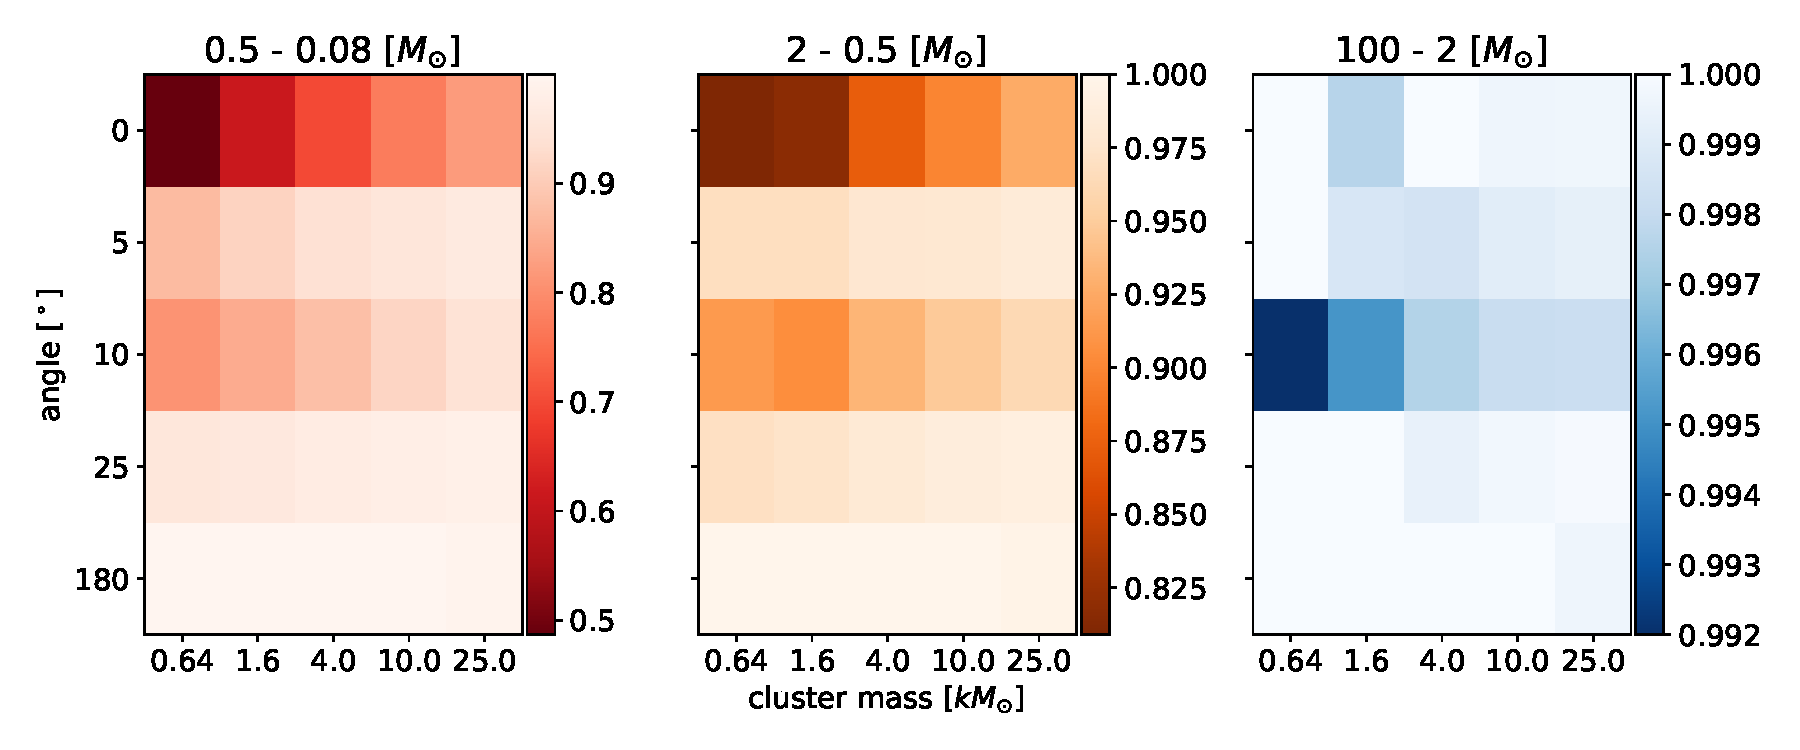
\includegraphics[width=\textwidth,height=\textheight,keepaspectratio]{Images/25_precision.pdf}
\end{figure}
\end{frame}

\begin{frame}
\begin{figure}
\centering
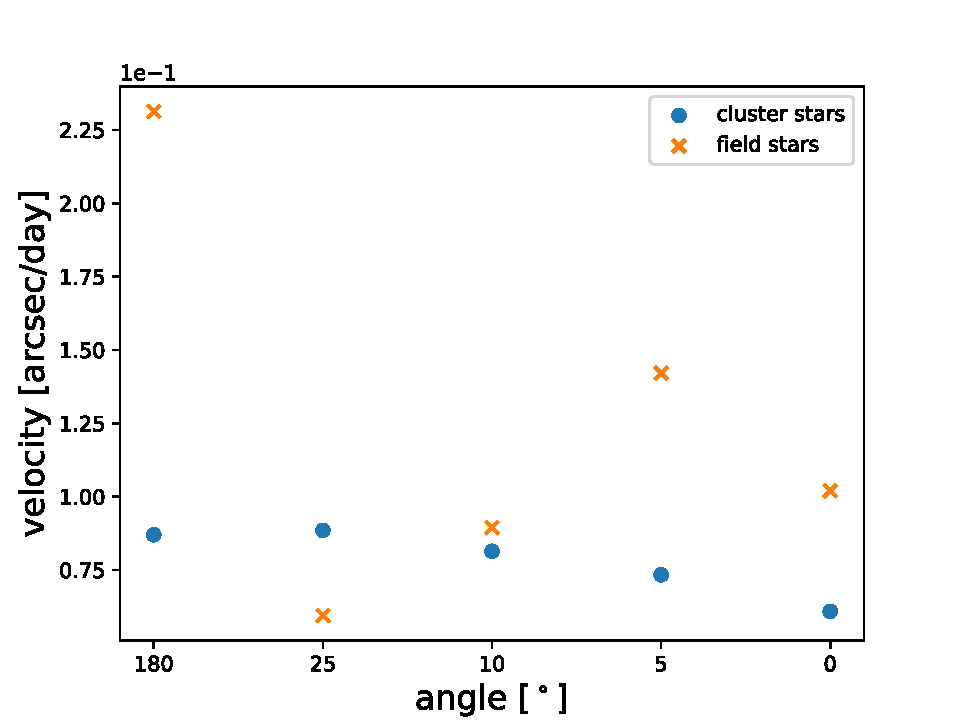
\includegraphics[width=\textwidth,height=\textheight,keepaspectratio]{Images/25_avg_vel_640.pdf}
\end{figure}
\end{frame}

\begin{frame}
\frametitle{general remarks on performance}
\begin{itemize}
\item Pass and loop by reference
\item Multithreading (OpenMP)
\item Choice of language
\item Define (mathematical) constants
\item C++ : emplace\_back VS push\_back
\end{itemize}
\end{frame}

\begin{frame}
\frametitle{Parameter optimization}
\begin{figure}
\centering
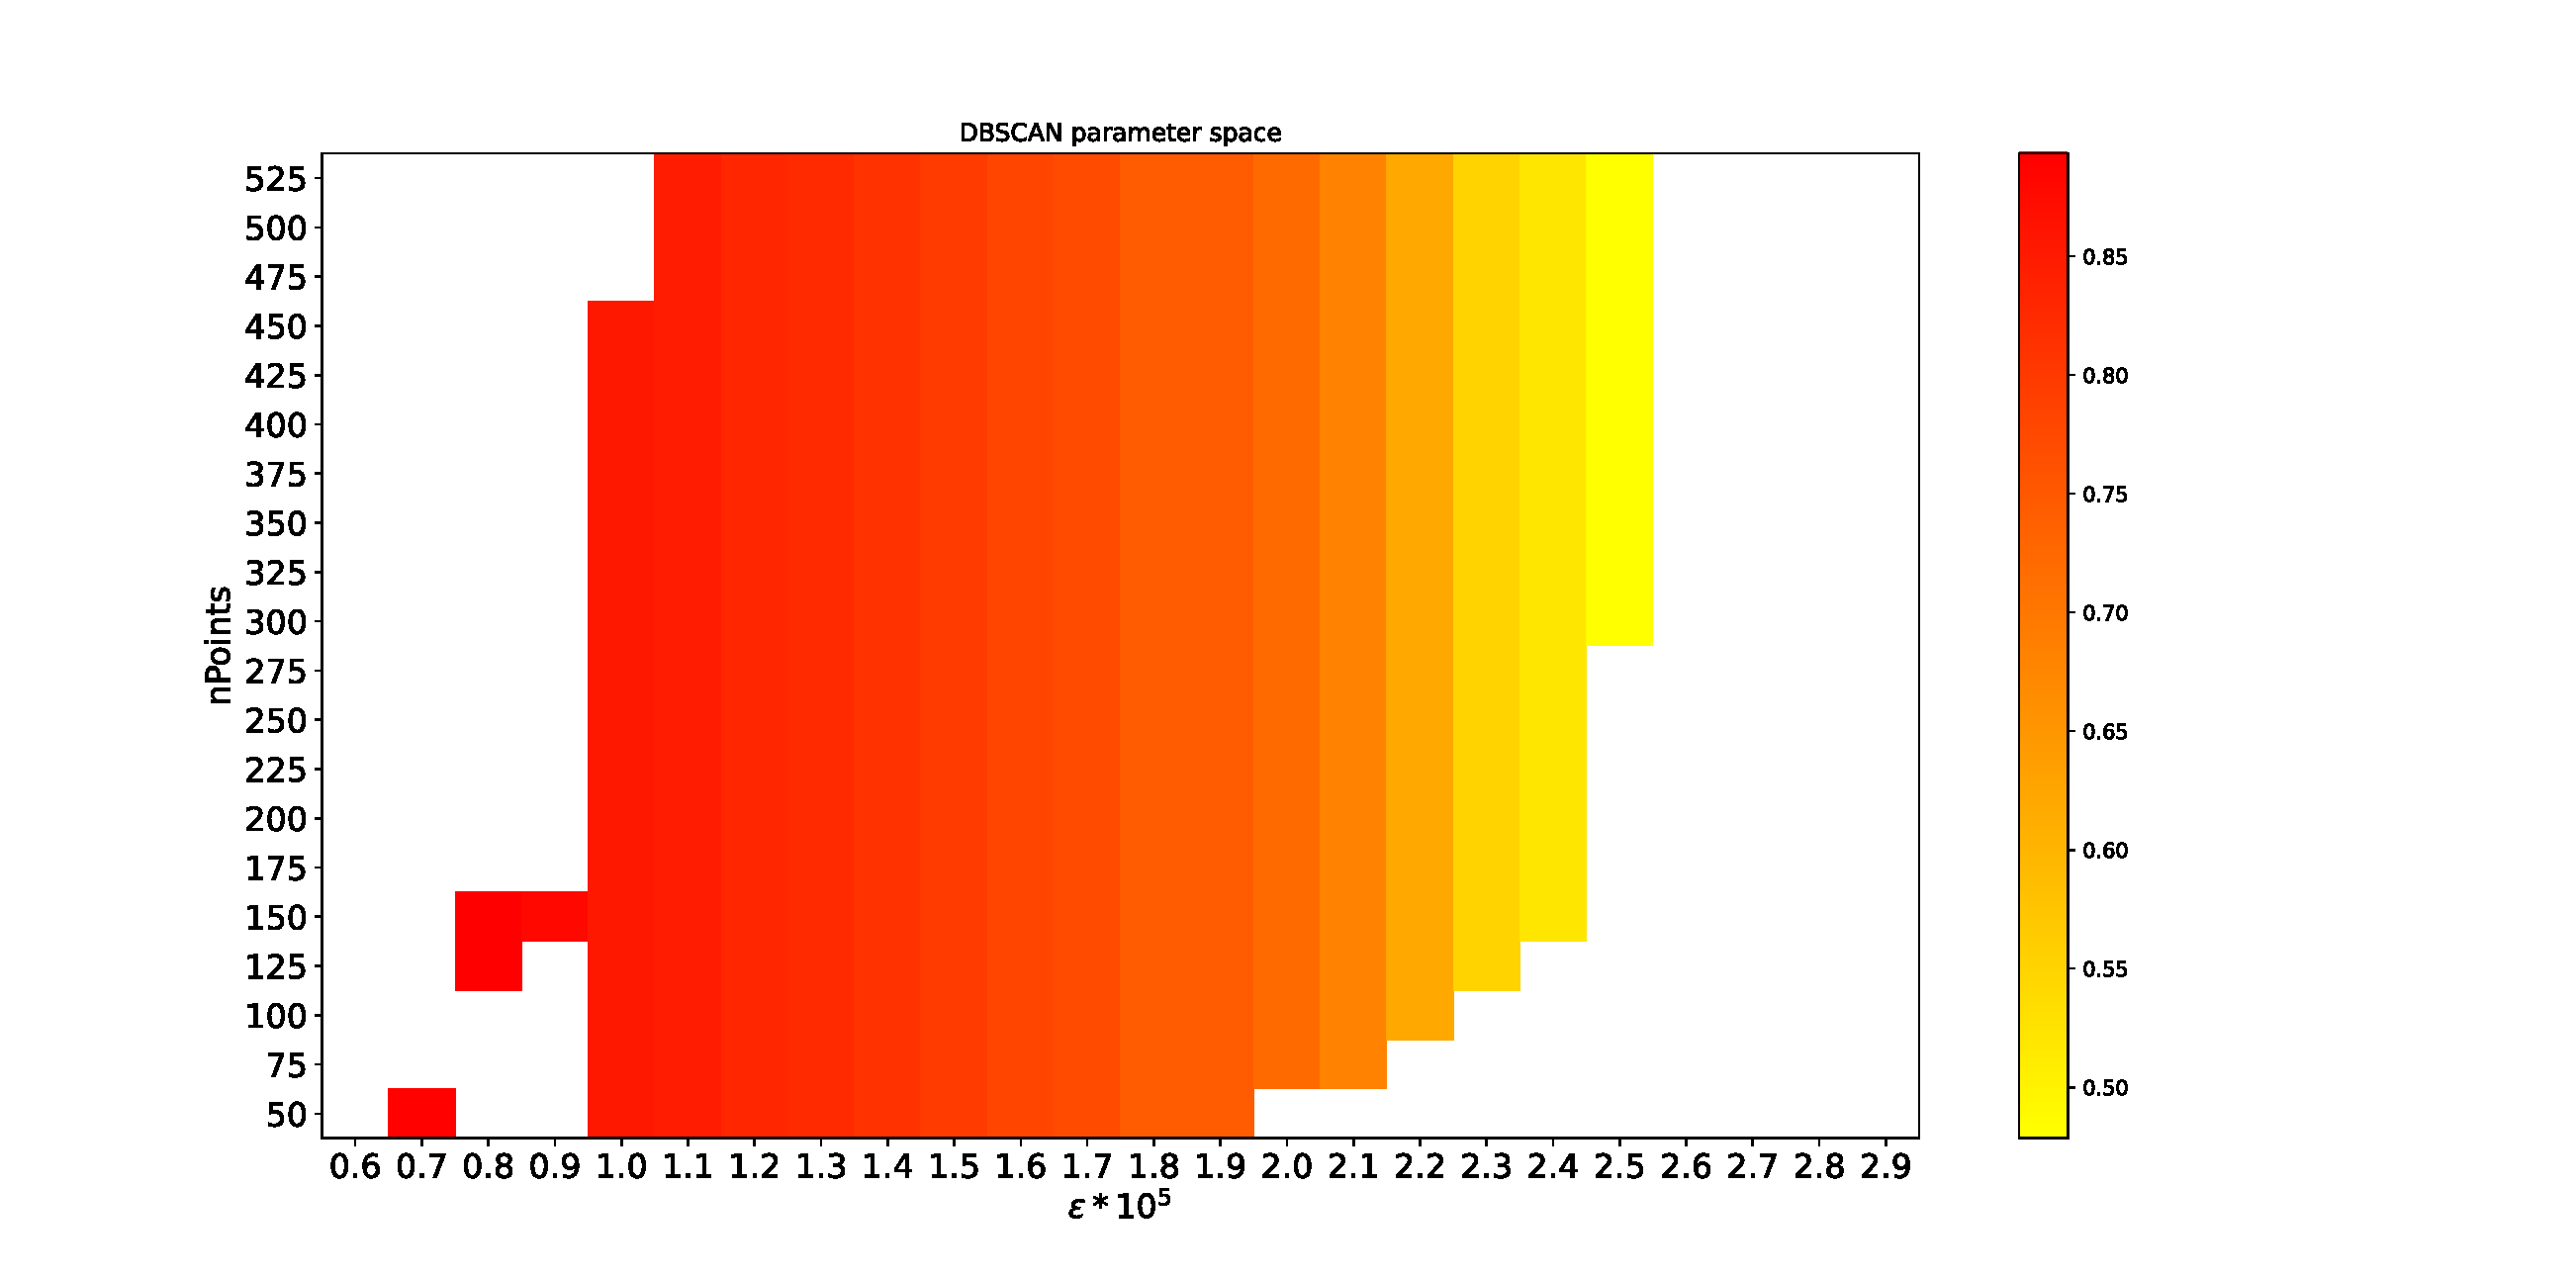
\includegraphics[width=\textwidth,height=\textheight,keepaspectratio]{Images/DBSCAN_parameter_space.pdf}
\end{figure}
\end{frame}























\end{document}